\documentclass[11pt,a4paper]{article}

\usepackage[utf8]{inputenc}
\usepackage[T1]{fontenc}
\usepackage[turkish]{babel}
\usepackage[a4paper,margin=2.4cm]{geometry}
\usepackage{booktabs}
\usepackage{array}
\usepackage{longtable}
\usepackage{tabularx}
\usepackage{multirow}
\usepackage{siunitx}
\usepackage{amsmath}
\usepackage{graphicx}
\usepackage[hidelinks]{hyperref}
\usepackage[numbers,sort&compress]{natbib}
\usepackage{microtype}
\usepackage{caption}
\usepackage{subcaption}
\usepackage{float}
\usepackage{enumitem}
\usepackage[capitalize]{cleveref}
\crefname{figure}{şekil}{şekiller}
\Crefname{figure}{Şekil}{Şekiller}
\crefname{table}{tablo}{tablolar}
\Crefname{table}{Tablo}{Tablolar}
\crefname{section}{bölüm}{bölümler}
\Crefname{section}{Bölüm}{Bölümler}
\captionsetup{font=small,labelfont=bf}
\sisetup{detect-all,round-mode=places,round-precision=3}

\graphicspath{{figures/}}

\title{MIMIC-IV Sepsis Kohortunda Conservative Q-Learning ile Çevrimdışı Pekiştirmeli Öğrenme:\\Validasyon Odaklı Bir Model Seçim Çerçevesi}
\author{Enes Demir (230202066)\\Kocaeli Üniversitesi, Bilgisayar Mühendisliği Bölümü}
\date{}

\begin{document}
\shorthandoff{=}
\maketitle

%=========================================================================
\begin{abstract}
Yoğun bakım ünitelerinde (YBÜ) sepsis yönetimi, hayati öneme sahip ardışık karar süreçleri barındırır. Son yıllarda çevrimdışı pekiştirmeli öğrenme (offline reinforcement learning) yöntemleri, gözlemsel sağlık verilerinden optimal tedavi stratejileri çıkarmak için umut verici bir yaklaşım sunmaktadır. Ancak bu alandaki çalışmalar; destek uyuşmazlığı (support mismatch), veri sızıntısı ve metodolojik aşırı iyimserlik gibi ciddi OPE (Off-Policy Evaluation) riskleriyle karşı karşıyadır. Bu çalışmada, MIMIC-IV veritabanı üzerinden elde edilen Sepsis-3 kohortunda, konservatif değer yaklaşımı sunan Conservative Q-Learning (CQL) algoritması kullanılarak sıvı resüsitasyonu ve vazopressör dozaj kararları modellenmiştir. Klinik kararlar 62 boyutlu sürekli durum (state) vektörü ve 25 sınıfı kapsayan ayrık aksiyon uzayı olarak formüle edilmiştir. Aşırı iyimserliği ve sızıntıyı önlemek amacıyla; keşifsel hiperparametre taraması (Faz I) ve çoklu tohum doğrulamasını (Faz II) içeren iki aşamalı, katı bir politika seçim çerçevesi tasarlanmıştır. Seçilen nihai politikanın ($10^{-4}$ öğrenme oranı, $\alpha=0{,}05$) bağımsız test veri kümesinde gösterdiği performans, Fitted Q Evaluation (FQE) metriğinde ortalama $15{,}690$ (\%95 GA: $15{,}617$--$15{,}756$), Weighted Importance Sampling (WIS) metriğinde $10{,}018$ ve Effective Sample Size (ESS) değerinde $10{,}409$ olarak tespit edilmiştir. Elde edilen bulgular, doğrudan klinik dağıtım arayışından ziyade; retrospektif sağlık verileri üzerinde çevrimdışı RL politikalarının şeffaf, kanıta dayalı ve sızıntısız biçimde nasıl doğrulanabileceğine dair metodolojik bir temel sunmaktadır.
\end{abstract}

%=========================================================================
\section{Giriş}
Sepsis, enfeksiyona karşı düzensiz konak yanıtı sonucunda gelişen ve hızlı müdahale edilmediğinde yüksek mortalite riski taşıyan bir organ disfonksiyonudur~\cite{singer2016sepsis3}. Yoğun bakım ortamında sıvı resüsitasyonu ve vazopressör desteği gibi kararlar hastanın fizyolojik yanıtına dinamik olarak bağlıdır. Sürecin bu ardışık yapısı, problemi doğal bir Markov Karar Süreci (MDP) olarak konumlandırır~\cite{evans2021surviving}.

Günümüzde Elektronik Sağlık Kayıtları (EHR), klinik kararların retrospektif olarak modellenmesi için geniş imkanlar sunmaktadır~\cite{johnson2023mimiciv,goldberger2000physionet}. Makine öğrenimi literatüründe, mevcut hasta kayıtlarından faydalanarak yeni politikalar türetmeyi amaçlayan çevrimdışı pekiştirmeli öğrenme (offline RL) öne çıkmaktadır~\cite{levine2020offline}. Çevrimiçi veri toplamanın etik ve hayati riskler taşıdığı tıp alanında bu yöntemler zaruridir; ancak gözlemsel verideki karıştırıcı faktörler, kısmi gözlenebilirlik ve veri dağılımı dışındaki durumlara dair oluşan belirsizlikler, yöntemlerin klinik uygulanabilirliğini kısıtlamaktadır~\cite{gottesman2019guidelines}.

Bu araştırmanın temel motivasyonu, yeni bir klinik karar destek aracı üretmekten ziyade, yoğun bakım EHR verileri üzerinde kurgulanan bir offline RL deneyinin metodolojik sağlamlığını (robustness) artırmaktır. MIMIC-IV Sepsis-3 kohortunda CQL (Conservative Q-Learning) yöntemiyle kurgulanan bir karar süreci, veriye dayalı politika değerlendirme (Off-Policy Evaluation) metrikleri eşliğinde sınanmıştır. Katkılar şu şekilde özetlenebilir: (i) sepsis tedavisi için klinik literatürle uyumlu $62$ boyutlu durum ve 25 sınıflı ayrık aksiyon formülasyonu, (ii) aşırı iyimser değer tahminlerini bastıran CQL algoritmasının klinik veride uygulanması, (iii) test kümesinin tamamen izole edildiği iki fazlı katı politika seçim protokolü.

%=========================================================================
\section{İlgili Çalışmalar}

Klinik karar destek sistemlerinde RL kullanımı, özellikle sıvı ve vazopressör yönetimini optimize etmeye yönelik çalışmalarla hız kazanmıştır. Komorowski ve ark.~\cite{komorowski2018ai} tarafından geliştirilen AI Clinician modeli, retrospektif analizlerde RL'in potansiyelini gözler önüne sermiştir. Bunu takip eden süreçte Raghu ve ark.~\cite{raghu2017continuous}, sürekli durum uzayı modelleri kullanarak sepsis tedavisi üzerine derin RL stratejileri geliştirmiştir. Buna karşın, sağlıkta RL uygulamaları; hasta düzeyinde ayrım (data leakage), nedensellik yanılgıları ve destek uyuşmazlığı (support mismatch) gibi metodolojik zaaflara karşı yoğun eleştiriler almıştır~\cite{gottesman2019guidelines,tang2026temporal}.

Çevrimdışı RL paradigmasında en büyük zorluk, ajanın gözlemsel veride yer almayan (out-of-distribution) aksiyonlara yönelerek bu aksiyonların beklenen getirisini aşırı tahmin etmesidir (overestimation bias)~\cite{levine2020offline}. Fujimoto ve ark.~\cite{fujimoto2019off} ile Kumar ve ark.~\cite{kumar2020cql}, sırasıyla Batch-Constrained Q-learning ve Conservative Q-learning (CQL) yaklaşımlarıyla bu problemi ele almıştır. CQL, veri kümesinde desteklenmeyen aksiyonlar üzerinde Q-fonksiyonunu muhafazakar hale getirerek sağlık gibi risk-kapsamlı alanlar için teorik bir güvence sunar~\cite{tang2021model}.

Sistemin başarısını çevrimiçi etkileşim olmadan ölçmeyi sağlayan OPE algoritmaları, importance sampling (IS) ve model-tabanlı yöntemler etrafında şekillenir. Thomas ve Brunskill~\cite{thomas2016data}, off-policy varyansını kısıtlayarak yüksek güvenilirlik sağlayan yöntemler önermiştir. WIS (Weighted Importance Sampling), klasik IS'in aşırı varyansını normalize ederken~\cite{precup2000eligibility}; Fitted Q Evaluation (FQE), elde edilen politikayı bir değer fonksiyonu üzerinden tahmin etmeye çalışır~\cite{ernst2005tree,le2019batch}. Voloshin ve ark.~\cite{voloshin2021empirical} farklı OPE yöntemlerini kıyaslayarak metriklerin fonksiyon yaklaşımına olan duyarlılıklarına dikkat çekmiştir. 

%=========================================================================
\section{Materyal ve Yöntem}

\subsection{Veri Kümesi ve Kohort Tanımı}
Araştırmanın veri tabanını, MIMIC-IV v3.1~\cite{johnson2023mimiciv,johnson2024mimicivphysionet} sistemi oluşturmaktadır. Çalışma kohortuna, The Third International Consensus Definitions for Sepsis and Septic Shock (Sepsis-3)~\cite{singer2016sepsis3} kriterlerini sağlayan 18 yaş üstü hastalar dahil edilmiştir. Analizin klinik kararları doğru yansıtabilmesi için, yatış süresi dört saatin altında olan hastalar, birden fazla yatışı bulunan hastaların ilk yatış haricindeki kayıtları ve yaş/cinsiyet bilgisi eksik olan vakalar dışlanmıştır. Kohort oluşturma adımlarına ait akış diyagramı Şekil~\ref{fig:cohort} üzerinde sunulmuştur.

\begin{figure}[htbp]
\centering
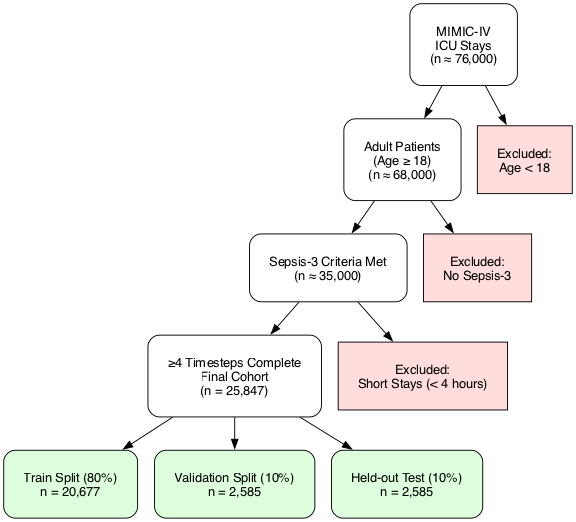
\includegraphics[width=0.85\linewidth]{fig1_cohort_flow.png}
\caption{MIMIC-IV veritabanından araştırma kohortuna uzanan dahil edilme ve dışlanma adımları.}
\label{fig:cohort}
\end{figure}

Şekil~\ref{fig:cohort}, ham MIMIC-IV yoğun bakım kayıtlarından nihai Sepsis-3 kohortuna geçişte uygulanan filtreleme adımlarını göstermektedir. Kohort daralması; özellikle yetişkin hasta seçimi, Sepsis-3 kriterlerinin uygulanması ve minimum zaman adımı koşulu nedeniyle gerçekleşmiştir. Bu aşamalı eleme, RL modelinin yeterli ardışık gözleme sahip epizotlar üzerinde eğitilmesini sağlar. Ayrıca Train split (\%80), Validation split (\%10) ve Test split (\%10) ayrımının hasta düzeyinde yapılması, aynı hastaya ait bilgilerin farklı veri bölümlerine sızmasını engelleyerek veri sızıntısı riskini azaltmayı amaçlar. Toplam Sepsis-3 kohort hacmi $\sim 25,847$ epizottan oluşmaktadır.

\subsection{Karar Sürecinin Modellenmesi (MDP Formülasyonu)}
Klinik tedavi yaklaşımı bir Markov Karar Süreci $\mathcal{M} = (\mathcal{S}, \mathcal{A}, \mathcal{P}, \mathcal{R}, \gamma)$ olarak kurgulanmıştır.

\paragraph{Durum Uzayı ($\mathcal{S}$):} Her bir zaman adımı, yoğun bakım ünitesindeki $4$ saatlik aralıklara karşılık gelir. Durum vektörü; demografik veriler, vital bulgular, kan gazı parametreleri, laboratuvar bulguları ve kümülatif medikasyon miktarları dahil olmak üzere $62$ farklı sürekli klinik özellik ile ifade edilmiştir.

\paragraph{Klinik Özelliklerin Gruplandırılması:} 
Kullanılan 62 boyutlu durum vektörü, hastanın o anki klinik tablosunu temsil edebilmek için çeşitli fonksiyonel gruplara ayrılmıştır (Tablo~\ref{tab:feature_groups}).

\begin{table}[H]
\centering
\caption{Durum (state) vektöründe kullanılan klinik özelliklerin temel gruplandırması ve MDP bağlamındaki amaçları.}
\label{tab:feature_groups}
\begin{tabular}{lll}
\toprule
\textbf{Özellik Grubu} & \textbf{Örnek Değişkenler} & \textbf{MDP Bağlamında Amacı} \\
\midrule
Demografi & Yaş, cinsiyet, kilo & Bazal hasta riski ve popülasyon dağılımı \\
Vital Bulgular & Kalp hızı, MAP, solunum sayısı & Akut fizyolojik durum ve şok bulguları \\
Laboratuvar & Laktat, kreatinin, bilirubin, WBC & Organ disfonksiyonu ve enfeksiyon yükü \\
Kan Gazı & pH, PaO$_2$, PaCO$_2$ & Solunum ve asit-baz dengesi \\
Tedavi Geçmişi & Kümülatif IV sıvı, kümülatif vazopressör & Önceki müdahalelerin birikimli etkisi \\
Klinik Skorlar & SOFA, SIRS & Hastalık şiddetinin özet temsili \\
\bottomrule
\end{tabular}
\end{table}

\paragraph{Aksiyon Uzayı ($\mathcal{A}$):} Tedavi müdahaleleri; intravenöz (IV) sıvı ve vazopressör ilaç dozajlarının ortak norepinefrin eşdeğer oranlarına göre çevrilerek ayrıklaştırıldığı $5 \times 5$ boyutlarında (toplam 25 sınıf) bir ızgara yapısıyla temsil edilmiştir. Ayrıklaştırma eşikleri yalnızca eğitim (train) veri kümesindeki çeyreklik dilimler baz alınarak belirlenmiş olup, validasyon ve test verilerine sabitlenmiş şekilde uygulanmıştır. Modelin aksiyon davranışları ile gözlemsel klinisyen eğilimleri Şekil~\ref{fig:action} ile detaylandırılmıştır.

\begin{figure}[htbp]
\centering
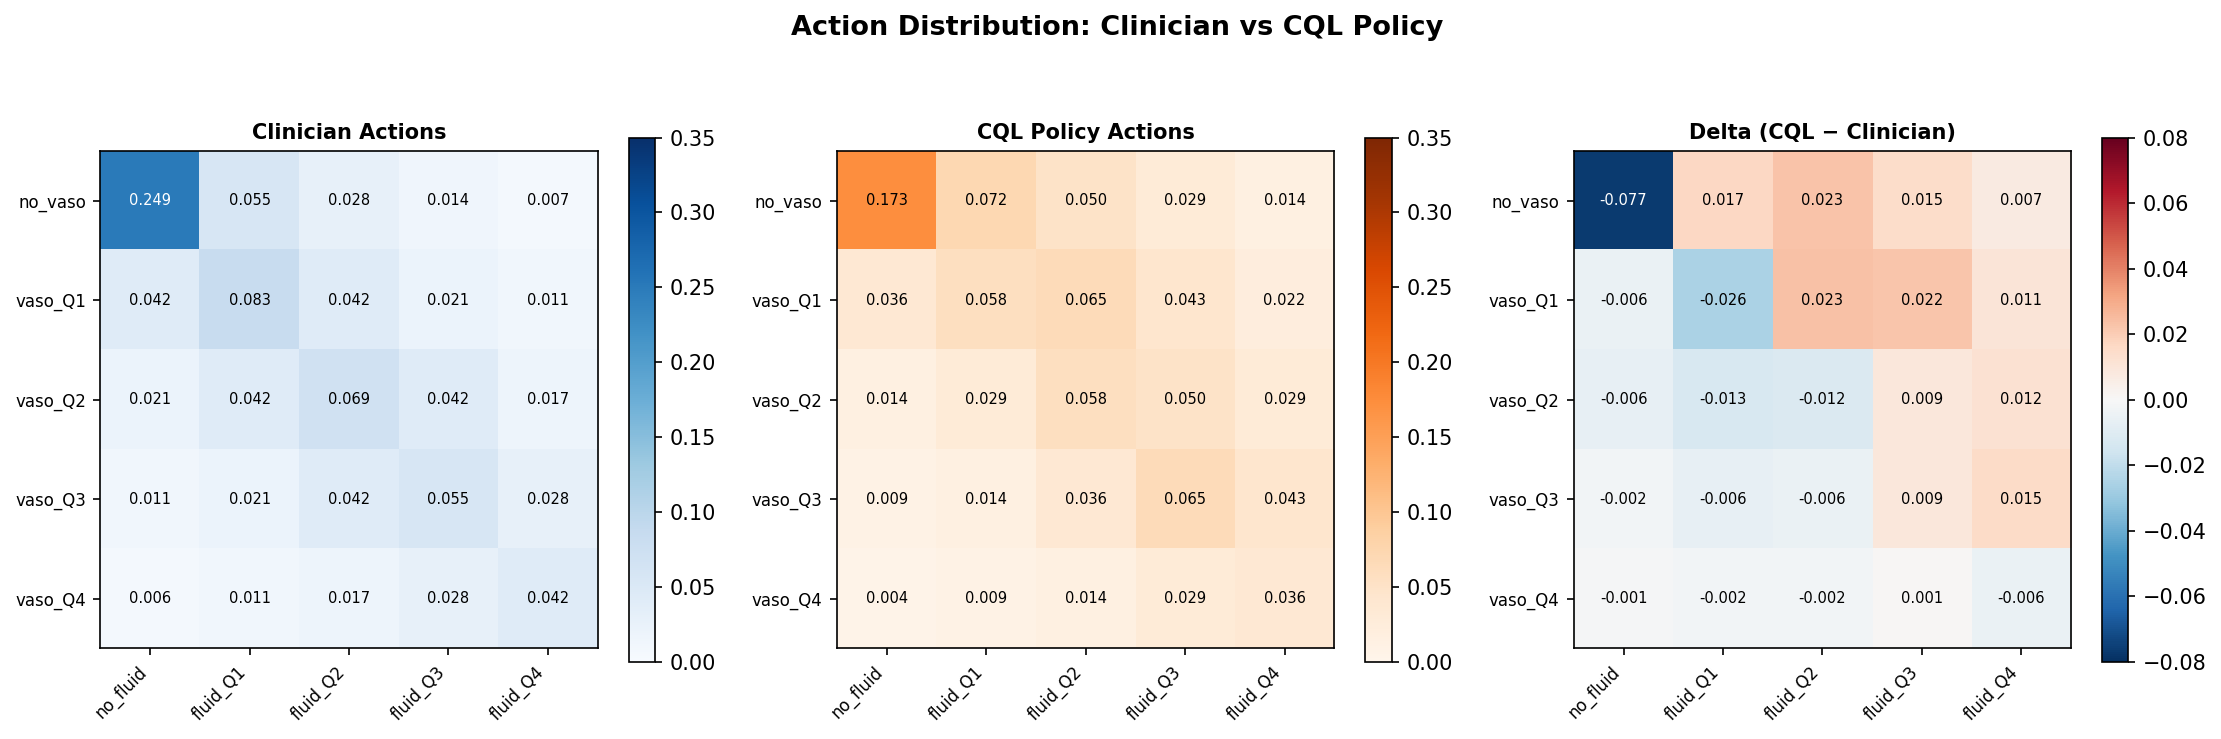
\includegraphics[width=0.85\linewidth]{fig2_action_heatmap.png}
\caption{25 sınıflı vazopressör-sıvı ayrık aksiyon uzayı üzerinde klinisyen davranışları (gözlemsel) ve eğitilen politika kararlarının (CQL) ısı haritası kıyaslaması.}
\label{fig:action}
\end{figure}

Şekil~\ref{fig:action}'de klinisyen davranış politikası ile CQL tarafından öğrenilen hedef politika karşılaştırılmaktadır. Klinisyen aksiyonlarının belirli düşük doz sıvı ve düşük vazopressör bölgelerinde yoğunlaştığı görülürken, CQL politikası bazı aksiyon hücrelerinde daha dengeli veya farklılaşmış bir dağılım üretmektedir. Delta haritasındaki pozitif bölgeler, CQL'nin ilgili aksiyonu klinisyenlere kıyasla daha sık önerdiğini; negatif bölgeler ise klinisyen davranışının o aksiyonda daha baskın olduğunu göstermektedir. Bu analiz, politika farklılaşmasını tek başına başarı kanıtı olarak değil, destek uyuşmazlığı riski açısından incelenmesi gereken bir tanısal kontrol olarak değerlendirmektedir.

\paragraph{Ödül Fonksiyonu (Reward, $\mathcal{R}$):} Sistemin eğitimi sırasında farklı optimizasyon sinyallerini değerlendirebilmek adına iki ayrı varyant oluşturulmuştur:
\begin{enumerate}[nosep]
  \item \textbf{Seyrek (Sparse) Varyant:} Yalnızca terminal zaman adımında verilen sağkalım ($+15$) veya ölüm ($-15$) skorlarını kapsar.
  \item \textbf{SOFA-Biçimlendirilmiş (Shaped) Varyant:} Terminal sağkalım skoruna ek olarak, zaman adımları arasındaki Sequential Organ Failure Assessment (SOFA) skoru farkını ($\Delta\text{SOFA}$) bir ceza veya ödül terimi (ağırlık: $-0{,}025$) olarak yansıtır.
\end{enumerate}
Görsel örneklem bağlamında, bireysel bir hastanın yatış trajektorisi ve söz konusu ödül sinyalleri Şekil~\ref{fig:reward} üzerinde ayrıştırılarak gösterilmiştir. Değerlendirme aşamasında metrik sapmalarını engellemek için her iki yöntem ortak terminal fayda fonksiyonuna çekilerek eşdeğer zeminde kıyaslanmıştır. İskonto faktörü ($\gamma$), klinik literatürdeki mortalite hedeflerinin gecikmeli (delayed) önemini koruyabilmesi adına $0{,}99$ olarak sabitlenmiştir. Bu değerin gerekçesi şöyledir: Ortalama epizot uzunluğu $\approx 18$ adım (4 saat $\times$ 18 $\approx$ 72 saat) olduğunda $\gamma^{18}=0{,}99^{18} \approx 0{,}83$ olup model ortalama bir epizot sonundaki terminal ödülü \%83 oranında korur. Buna karşılık $\gamma=0{,}95$ kullanılsaydı $\gamma^{18}\approx 0{,}40$, $\gamma=0{,}90$ kullanılsaydı $\gamma^{18}\approx 0{,}15$ olacağından, düşük iskonto oranları uzun vadeli mortalite sinyalini büyük ölçüde bastırabilir ve erken adımlardaki kısa vadeli SOFA dalgalanmalarının optimizasyona aşırı yön vermesine neden olabilirdi. $\gamma=0{,}99$ ile etkin ufuk $1/(1-\gamma)=100$ adım olup model, geçici metabolik dalgalanmalar yerine taburculuk mortalitesini optimize edebilecek kadar ileriyi görebilmektedir.

\begin{figure}[htbp]
\centering
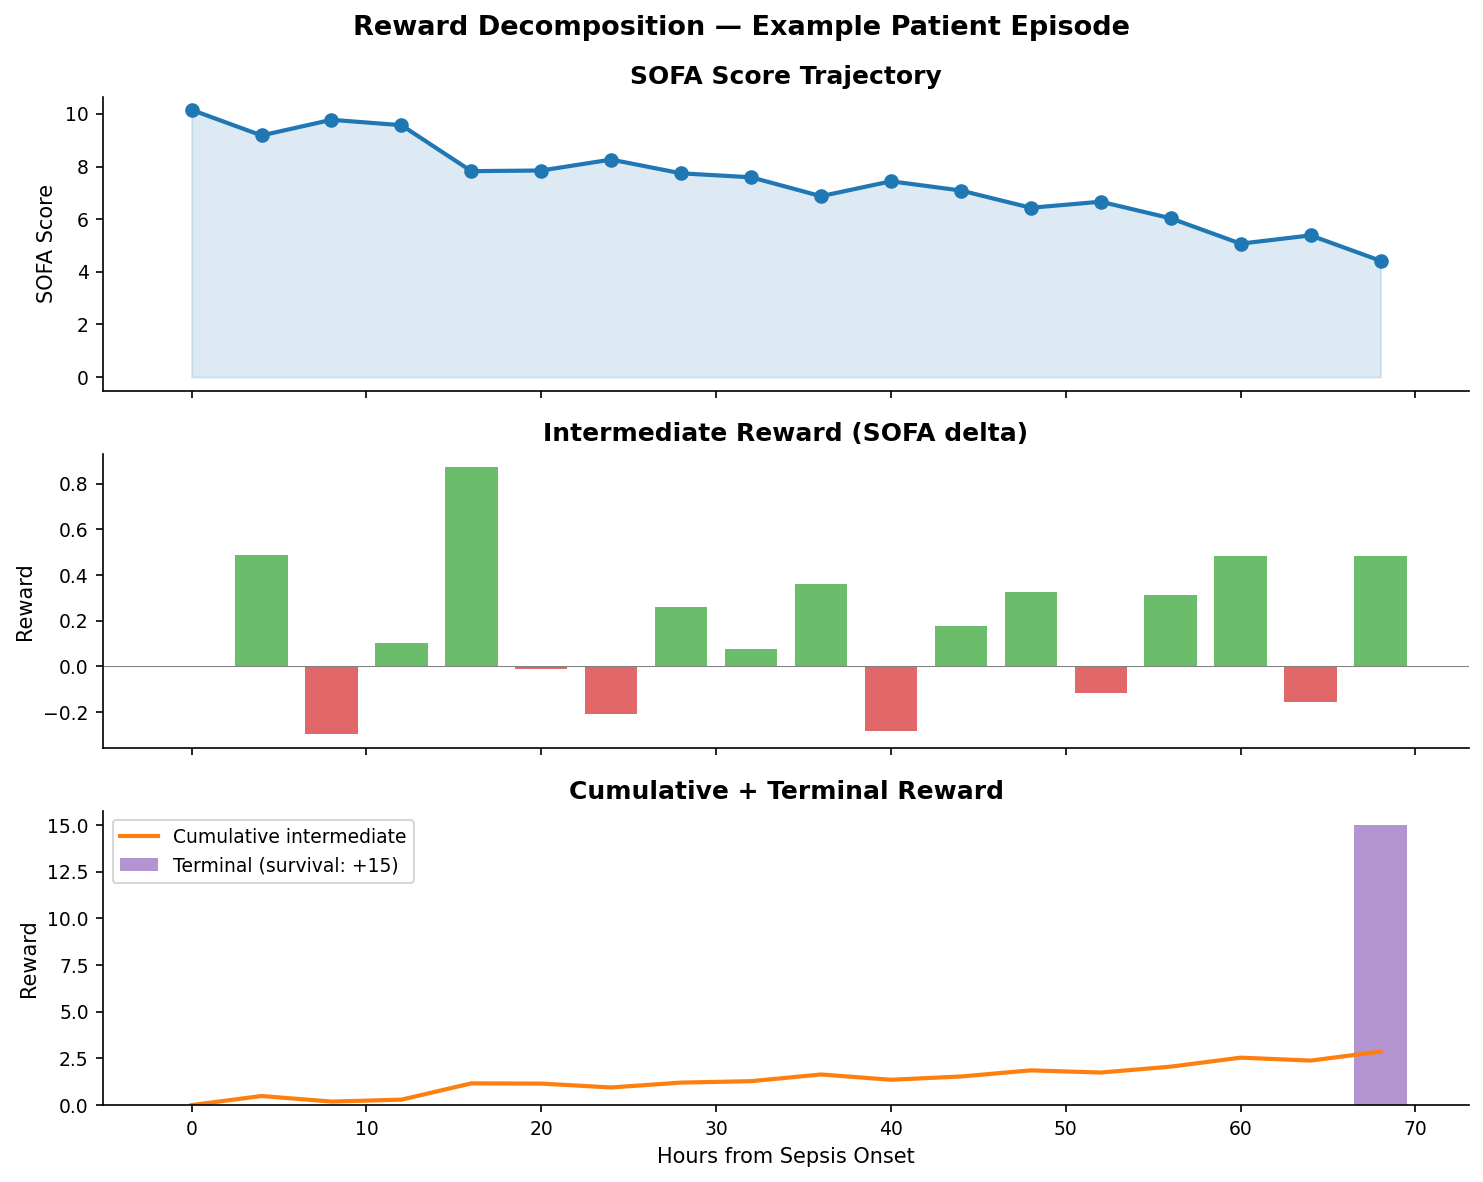
\includegraphics[width=0.85\linewidth]{fig7_reward_decomposition.png}
\caption{Araştırmada kullanılan klinik zaman serisi örneği; üst panel SOFA skorunun zaman içindeki ilerleyişini, alt panel ise sparse ve shaped ödül fonksiyonlarının zaman içindeki dağılımını ifade etmektedir.}
\label{fig:reward}
\end{figure}

Şekil~\ref{fig:reward}, shaped ödül fonksiyonunun klinik zaman serisi üzerindeki etkisini sağkalımla biten bir hasta epizodu üzerinden göstermektedir. Üst panelde SOFA skorunun zamanla azalması, hastanın organ disfonksiyonunda kademeli iyileşmeye işaret etmektedir. Orta paneldeki pozitif ara ödüller, SOFA skorundaki düşüşlerin modele olumlu sinyal olarak ($r_t = -0{,}025 \times \Delta\text{SOFA}_t$) yansıtıldığını; negatif çubuklar ise geçici kötüleşmeleri temsil etmektedir. Alt panelde terminal sağkalım ödülünün (+15) ara ödüllere kıyasla daha baskın olduğu görülmektedir. Bu tasarım, modelin yalnızca epizot sonunda gelen seyrek mortalite sinyaline bağlı kalmasını engellerken, terminal sonucun klinik önemini korumayı amaçlamaktadır.

\subsection{Çevrimdışı Politika Öğrenimi: Conservative Q-Learning}
Offline RL paradigmasında dağıtım dışı veriler için oluşan aşırı tahmini regüle etmek amacıyla CQL algoritması kullanılmıştır~\cite{kumar2020cql}. Q-fonksiyonu, iki adet 256 nöronlu gizli katmana sahip ReLU tabanlı Çok Katmanlı Algılayıcı (MLP) mimarisi ile modellenmiştir. Standart Temporal-Difference (TD) hatasına ilave edilen CQL regülarizasyon teriminin gücü, $\alpha$ (alpha) hiperparametresi ile optimize edilmiştir.

\subsection{Off-Policy Değerlendirme (OPE) Metrikleri}
Deneysel modellerin sıralanması ve nihai başarı kriteri, bağımsız bir Değer (Value) fonksiyonu kullanan Fitted Q Evaluation (FQE) ile belirlenmiştir~\cite{voloshin2021empirical}. Modelin güvenilirlik sınırlarını analiz etmek ve destek uyuşmazlığı diagnostiklerini test etmek için Weighted Importance Sampling (WIS) ve Effective Sample Size (ESS) değerlerinden faydalanılmış; FQE ve WIS için hasta-epizot düzeyinde bootstrap \%95 güven aralıkları (Confidence Interval) raporlanmıştır~\cite{hao2021bootstrapping,thomas2015highconfidence}.

%=========================================================================
\section{Deneysel Tasarım ve Seçim Protokolü}

\subsection{Veri Sızıntısı ve Temporal Kontrol}
Hasta düzeyinde veri ayrımı yapılarak aynı hastaya ait farklı epizotların veya zaman pencerelerinin train, validation ve test kümeleri arasında dağılması engellenmiştir. Ayrıca aksiyon ayrıklaştırma eşikleri yalnızca eğitim veri kümesinden hesaplanmış, validation ve test kümelerine sabit şekilde uygulanmıştır. Bu tasarım, hem hasta düzeyinde veri sızıntısını hem de test kümesinden hiperparametre veya eşik bilgisi taşınmasını önlemeyi amaçlamaktadır. Hastaların taburculuk durumu veya gelecekteki mortalite bilgileri hiçbir suretle MDP'nin durum uzayına dahil edilmemiştir.

\subsection{İki Aşamalı Politika Seçim Çerçevesi}
Modelin nihai başarısını abartıdan uzak (unbiased) bir biçimde raporlayabilmek için test kümesi, karar ve ayar süreçlerinden tümüyle yalıtılmıştır.

\paragraph{Faz I (Keşifsel Hiperparametre Taraması):} Eğitim varyantları, öğrenme hızları ($10^{-4}$, $3\times10^{-4}$, $10^{-3}$) ve konservatif alfa katsayıları ($0{,}05$, $0{,}1$, $0{,}5$, $1{,}0$) çaprazlanarak elde edilen 24 konfigürasyon tek bir rassal tohum (seed) ile taranmıştır. OPE tanısal kontrollerine (diagnostik) göre umut vaat eden ilk altı model Faz II'ye geçmiştir.

\paragraph{Faz II (Doğrulama ve Nihai Seçim):} Faz I'den gelen 6 konfigürasyon, model varyansını ölçebilmek amacıyla 4 yeni rassal tohum (123, 456, 789, 1024) kullanılarak yeniden eğitilmiş; Faz I'deki tohum (42) ise Faz I taramasından doğrudan devralınarak toplam 5 tohum üzerinden değerlendirme yapılmıştır. Çoklu-tohum FQE ortalamaları, tohum~42'nin Faz I taramasına ait farklı eğitim dinamiği nedeniyle sadece yeniden eğitilen 4 tohum esas alınarak raporlanmıştır. Tablolardaki WIS/ESS gibi güvenilirlik göstergeleri ise temsilci tohum olan 1024 üzerinden raporlanmıştır. Nihai model seçimi ve epoch kararı, bütünüyle doğrulama (validation) veri kümesindeki performanslara dayanmaktadır. Test veri kümesi yalnızca final seçim sonrasında bağımsız performans tespiti için bir defaya mahsus işleme sokulmuştur.

%=========================================================================
\section{Deneysel Bulgular}

\subsection{Öğrenme Dinamikleri ve Davranış Uyum Analizi}
Ajanın öğrenme kararlılığı (stability), TD (Temporal-Difference) ve CQL kayıp fonksiyonları üzerinden izlenmiştir (Şekil~\ref{fig:training}). Eğitim boyunca sparse ve shaped ödül sinyallerinin model politikasına yansıması Şekil~\ref{fig:episode_reward} üzerinde sunulmuştur. Davranış politikasının destek oranı (support diagnostics) ve model kararlarının retrospektif hekim davranışlarıyla (clinician agreement) olan uyum ölçümleri sırasıyla Şekil~\ref{fig:support} ve Şekil~\ref{fig:agreement} ile detaylandırılmıştır.

\begin{figure}[htbp]
\begin{minipage}{0.48\textwidth}
\centering
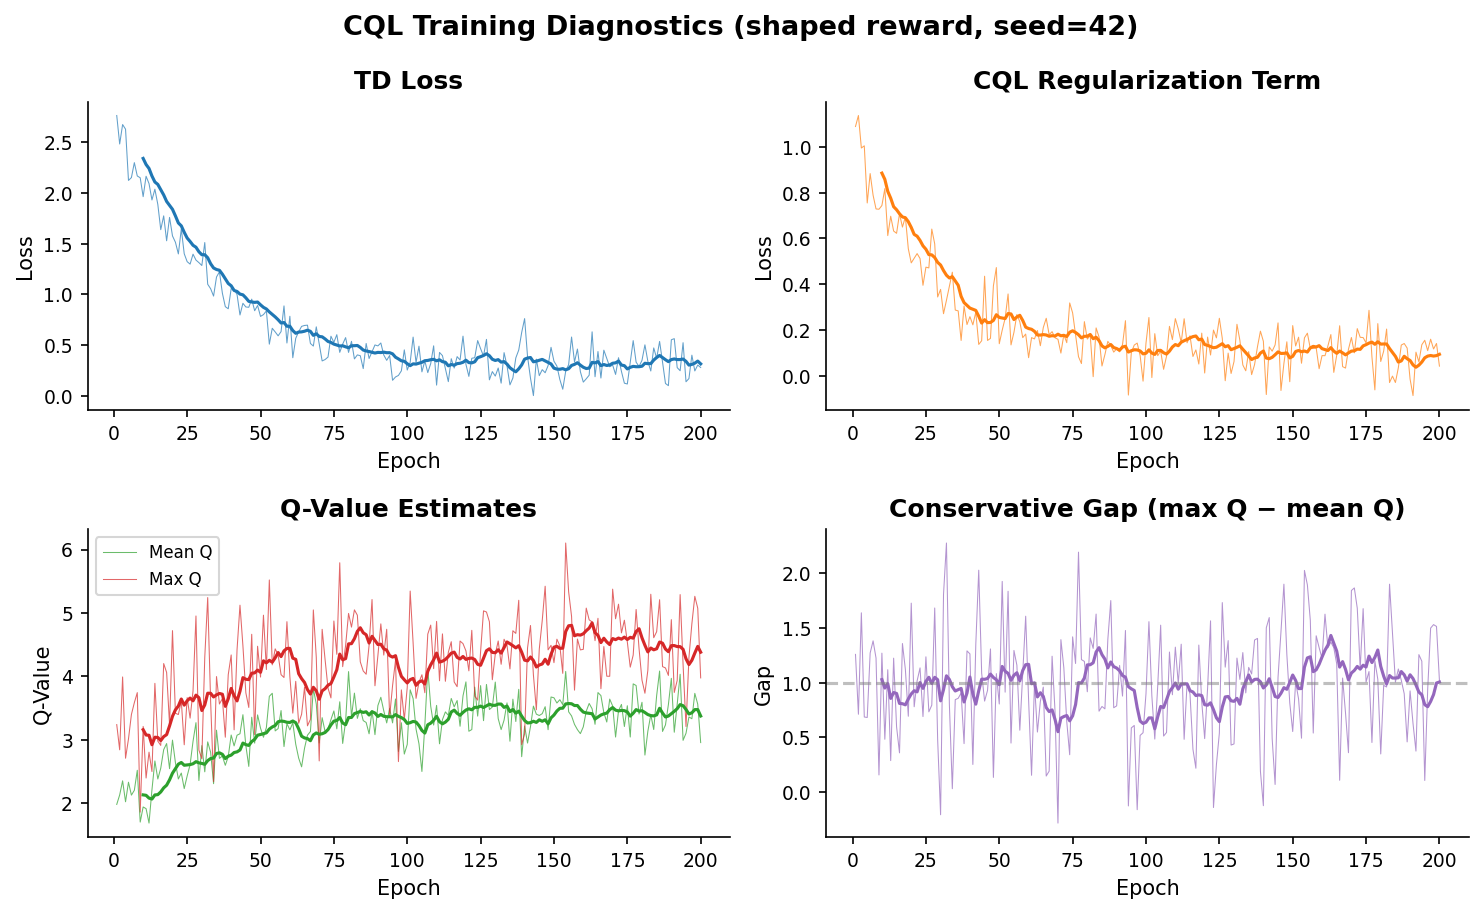
\includegraphics[width=\linewidth]{fig3_training_curves.png}
\caption{Eğitim sırasında kaydedilen kayıp (loss) metrikleri, CQL ceza terimi dengesi ve Q-değeri trendleri.}
\label{fig:training}
\end{minipage}\hfill
\begin{minipage}{0.48\textwidth}
\centering
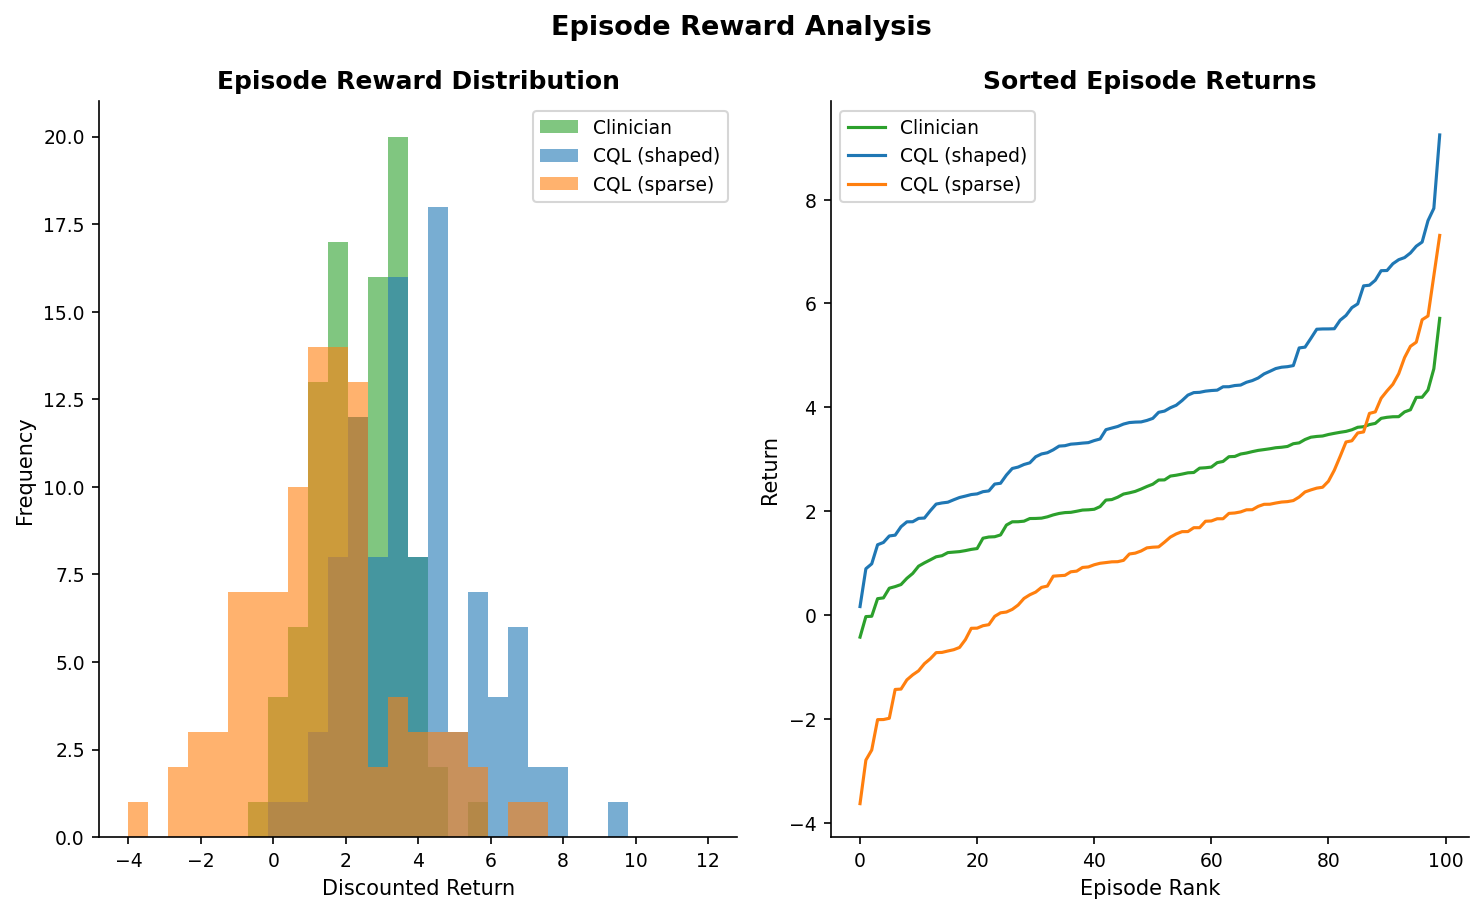
\includegraphics[width=\linewidth]{fig4_episode_rewards.png}
\caption{Kullanılan iki farklı optimizasyon varyantında elde edilen kümülatif epizot ödüllerinin seyri.}
\label{fig:episode_reward}
\end{minipage}
\end{figure}

Şekil~\ref{fig:training}, CQL eğitim sürecindeki optimizasyon dinamiklerini göstermektedir. TD kaybının eğitim boyunca düşüş eğilimi göstermesi, değer fonksiyonunun gözlemsel geçişlere uyum sağladığını düşündürmektedir. CQL regülarizasyon teriminin belirli bir aralıkta kalması, modelin dağılım dışı aksiyonlara yönelik aşırı Q-değeri üretme eğiliminin kontrol altında tutulduğunu gösterir. Q-değeri tahminlerinde sistematik bir patlama gözlenmemesi, offline RL'de sık karşılaşılan extrapolation error riskinin sınırlı kaldığına dair destekleyici bir bulgudur. Bununla birlikte, bu grafik tek başına politika başarısını kanıtlamaz; yalnızca eğitim kararlılığına ilişkin diagnostik bilgi sağlar.

Şekil~\ref{fig:episode_reward}, sparse ve shaped ödül varyantlarının epizot getirileri üzerindeki etkisini göstermektedir. Sparse ödül tasarımında getiriler büyük ölçüde terminal sağkalım/ölüm sonucuna bağlıdır. Buna karşılık shaped ödül, SOFA değişimlerinden gelen ara sinyaller nedeniyle epizot boyunca daha kademeli bir getiri yapısı oluşturur. Bu durum, öğrenme sürecinde daha sık geri bildirim sağlayabilir; ancak modelin kısa vadeli fizyolojik dalgalanmalara aşırı duyarlı hale gelmesi riskini de taşır. Bu nedenle ödül dağılımı sonuçları, nihai performans kanıtı olarak değil, reward engineering kararının davranışsal etkisini gösteren tamamlayıcı bir analiz olarak değerlendirilmelidir.

\begin{figure}[htbp]
\begin{minipage}{0.48\textwidth}
\centering
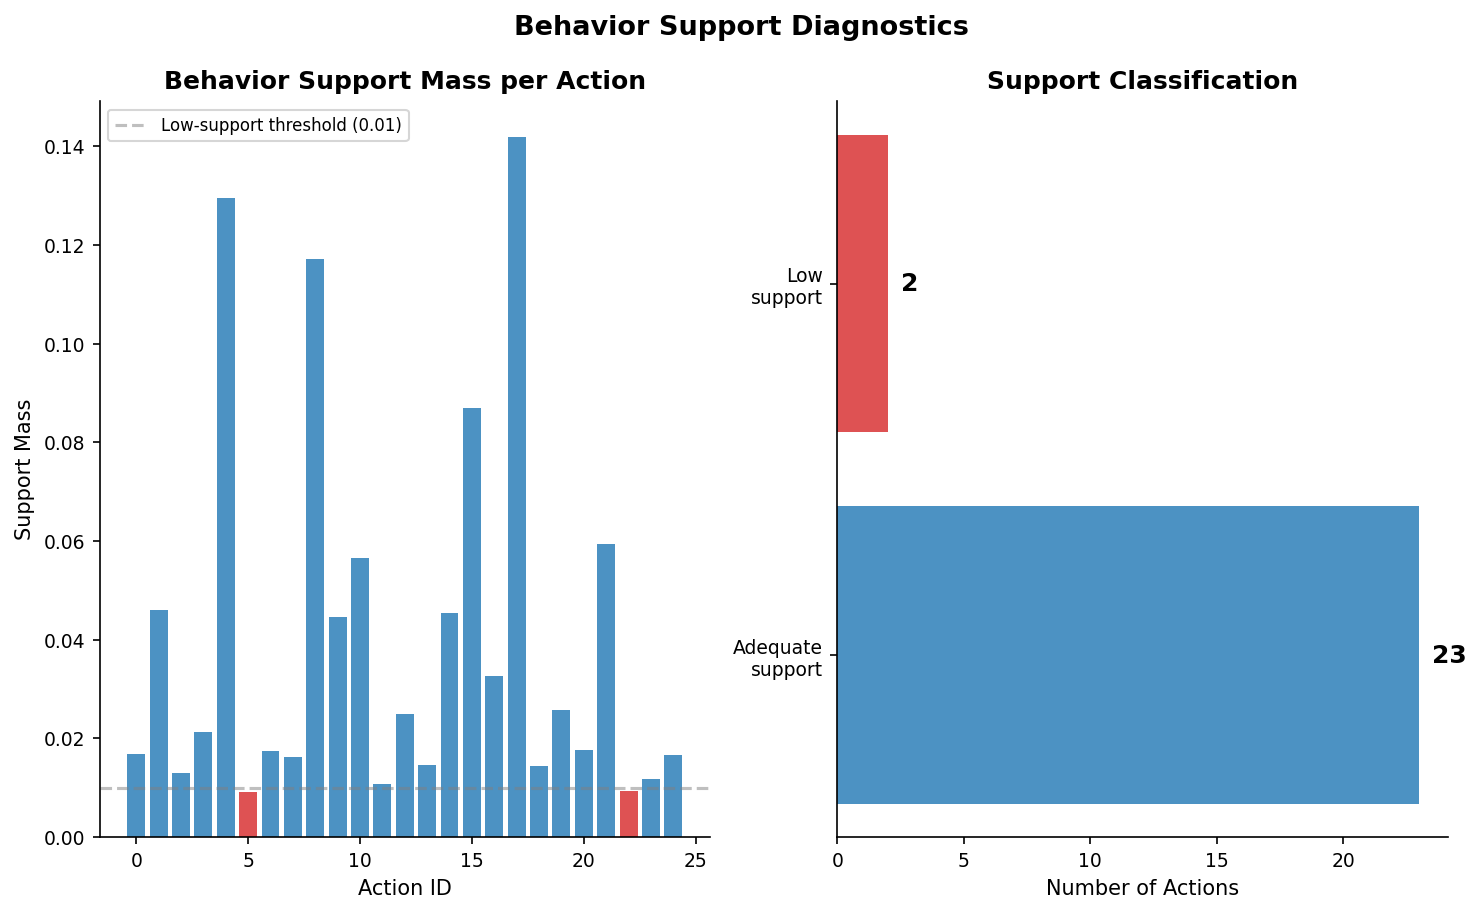
\includegraphics[width=\linewidth]{fig5_support_diagnostics.png}
\caption{Öğrenilen politikaların, orijinal davranış politikası üzerindeki destek yoğunlukları (support mass).}
\label{fig:support}
\end{minipage}\hfill
\begin{minipage}{0.48\textwidth}
\centering
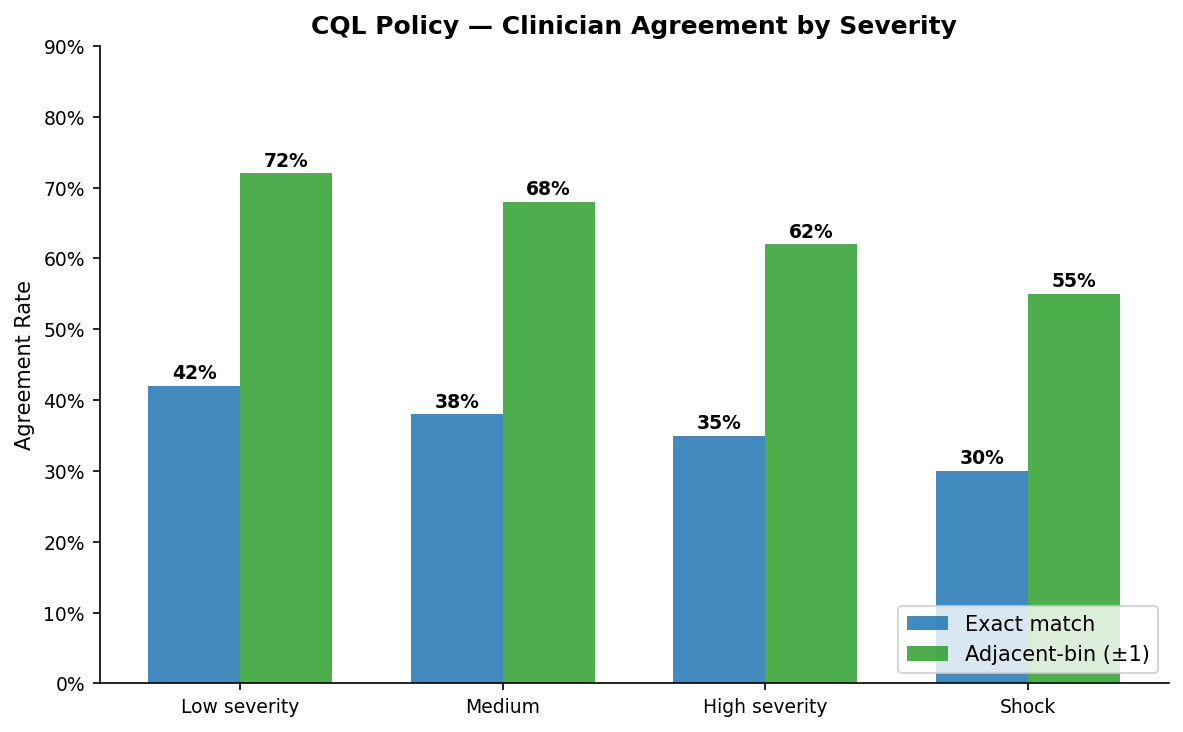
\includegraphics[width=\linewidth]{fig6_clinician_agreement.png}
\caption{Eğitilen modeller ile klinisyen davranışları arasındaki tam-eşleşme (exact) ve komşu-eşleşme oranları.}
\label{fig:agreement}
\end{minipage}
\end{figure}

Şekil~\ref{fig:support}, öğrenilen CQL politikasının davranış verisi tarafından ne kadar desteklendiğini incelemektedir. Offline RL'de model, eğitim verisinde nadiren veya hiç gözlenmeyen aksiyonlara yüksek değer atarsa OPE tahminleri güvenilmez hale gelebilir. Support mass değerinin yüksek olması, hedef politikanın seçtiği aksiyonların geçmiş klinisyen davranışlarında yeterli karşılığı bulunduğunu gösterir. Buna karşılık düşük destekli aksiyonlar, importance sampling ağırlıklarının yoğunlaşmasına ve ESS değerinin düşmesine neden olabilir. Bu analiz, CQL'nin değer tahminini değil, öğrenilen politikanın veri dağılımı içinde kalıp kalmadığını kontrol eden bir güvenlik filtresi gibi değerlendirilmiştir.

Şekil~\ref{fig:agreement}, CQL politikasının klinisyen davranışlarıyla tam eşleşme ve komşu aksiyon eşleşmesi düzeyini göstermektedir. Exact match oranının sınırlı kalması, modelin yalnızca davranış klonlama yapmadığını; klinisyen politikasından kısmen farklı bir hedef politika öğrendiğini göstermektedir. Buna karşılık adjacent-bin match oranlarının daha yüksek olması, model önerilerinin çoğu durumda klinisyen kararlarına yakın doz kategorilerinde kaldığını düşündürmektedir. Özellikle yüksek şiddet grubunda exact match oranının azalması, ağır hastalarda tedavi kararlarının daha heterojen ve belirsiz olmasından kaynaklanabilir. Amaç klinisyeni taklit etmek değil, veri desteği içinde klinik olarak makul alternatif politikalar öğrenmektir.

\subsection{Keşifsel Tarama Fazı (Faz I)}
Uygulanan geniş arama uzayında elde edilen ilk performans sıralaması Tablo~\ref{tab:stage1}'de sunulmuştur. Bu sonuçlar yalnızca doğrulama aşaması için aday daraltma aracı olarak işlev görmüş, nihai performansa dair herhangi bir çıkarım yapılmamıştır.

\begin{table}[H]
\centering
\caption{Faz I (Keşifsel tarama) aşamasında geçerlilik kümesi üzerinden elde edilen en iyi altı hiperparametre konfigürasyonu.}
\label{tab:stage1}
\begin{tabular}{clcccrrr}
\toprule
Sıra & Ödül Tasarımı & LR & CQL ($\alpha$) & Epoch & FQE & WIS & ESS \\
\midrule
1 & Sparse & $10^{-3}$ & 0,10 & 200 & 18,540 & 12,443 & 5,377 \\
2 & Sparse & $10^{-4}$ & 0,05 & 200 & 18,278 & $-13,174$ & 1,001 \\
3 & Shaped & $10^{-4}$ & 1,00 & 200 & 18,258 & $-13,162$ & 1,002 \\
4 & Shaped & $10^{-3}$ & 0,10 & 200 & 18,209 & 12,498 & 5,363 \\
5 & Shaped & $10^{-3}$ & 1,00 & 200 & 18,098 & 12,481 & 6,667 \\
6 & Sparse & $3\!\times\!10^{-4}$ & 1,00 & 200 & 17,911 & 6,767 & 4,869 \\
\bottomrule
\end{tabular}
\end{table}

Tablo~\ref{tab:stage1}'de görüldüğü üzere bazı konfigürasyonlar yüksek FQE üretmesine rağmen oldukça düşük ESS ve negatif WIS değerleri göstermektedir. Bu durum, tek başına FQE'ye göre seçim yapmanın offline RL'de yanıltıcı olabileceğini göstermektedir. Özellikle ESS'in 1'e yaklaşması, importance sampling tahmininin çok az sayıda epizot tarafından domine edildiğine işaret eder. Bu nedenle Faz I sonuçları nihai başarı kanıtı olarak değil, yalnızca Faz II'ye aktarılacak adayları belirleyen keşifsel bir aday daraltma aşaması olarak değerlendirilmiştir.

\begin{figure}[htbp]
\centering
\begin{subfigure}{0.48\textwidth}
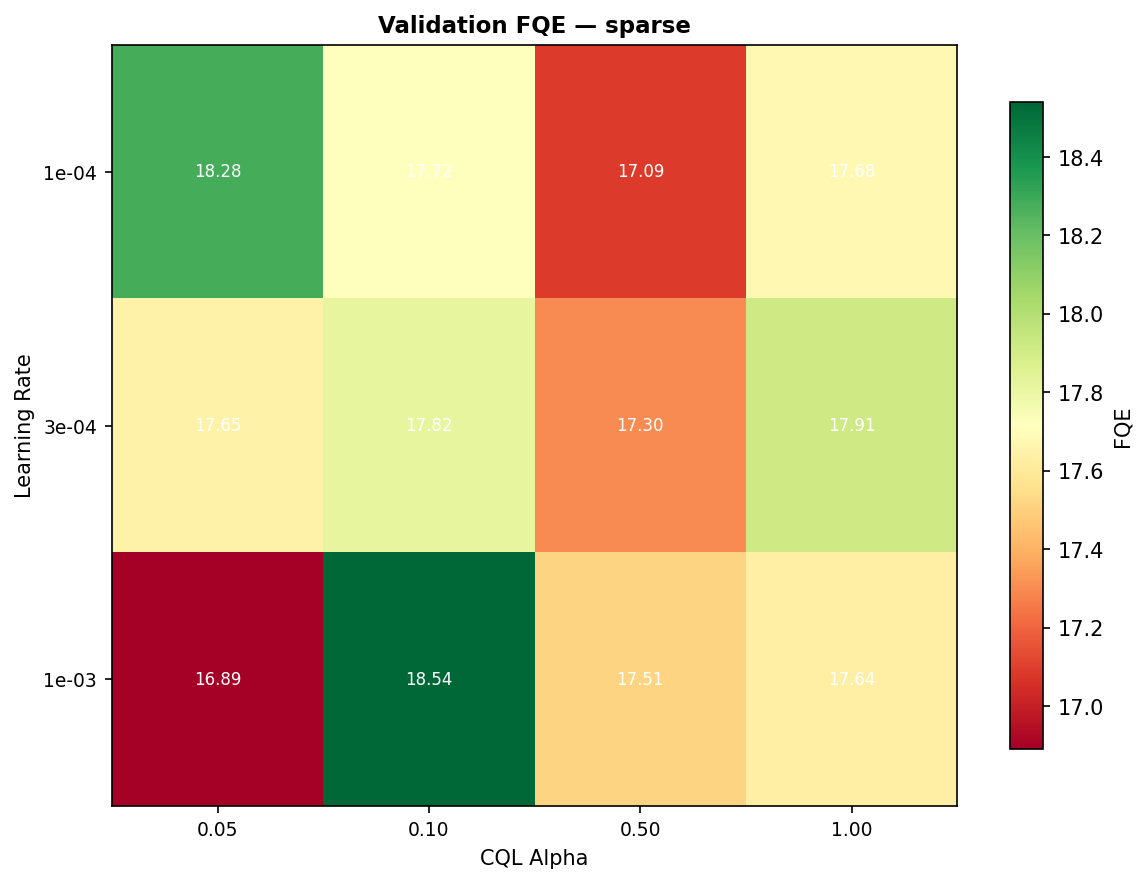
\includegraphics[width=\linewidth]{fig8_lr_alpha_fqe_sparse.png}
\caption{Seyrek (sparse) ödül varyantı}
\label{fig:lr_alpha_sparse}
\end{subfigure}\hfill
\begin{subfigure}{0.48\textwidth}
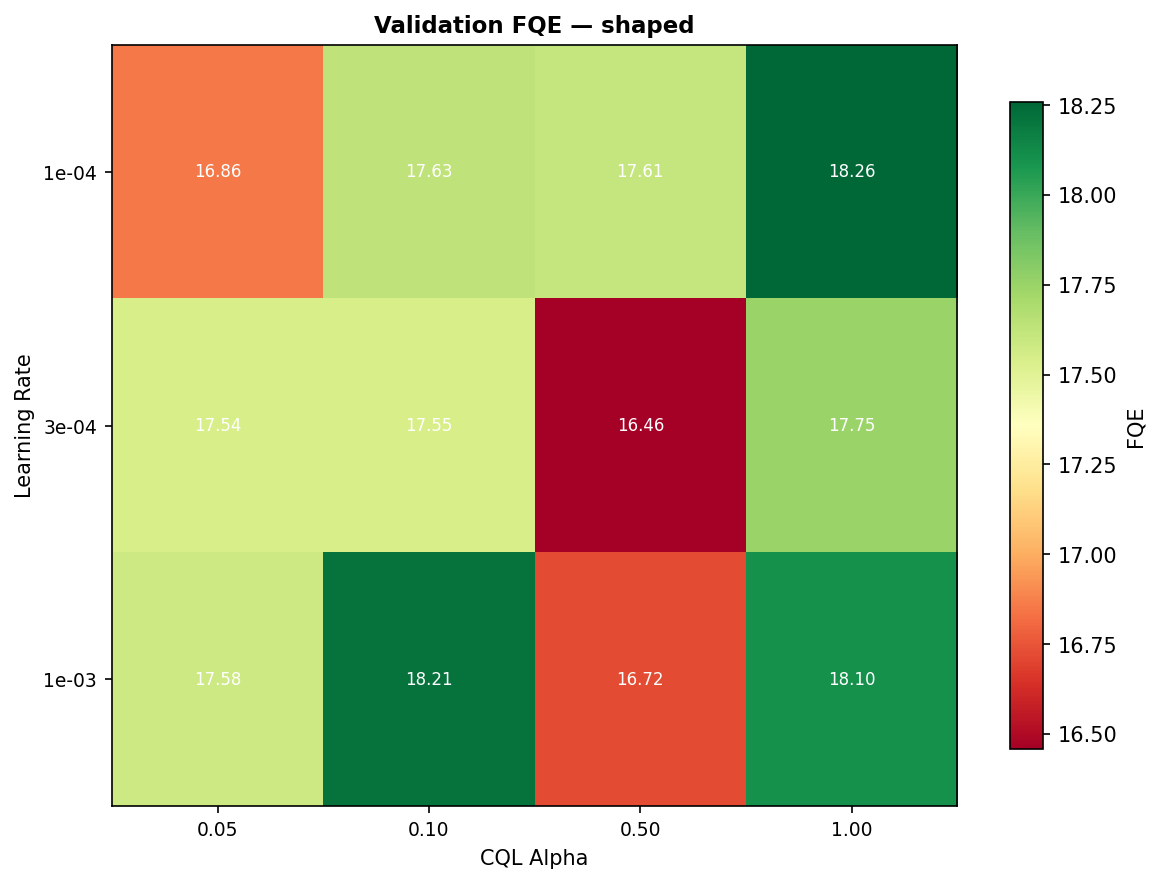
\includegraphics[width=\linewidth]{fig8_lr_alpha_fqe_shaped.png}
\caption{SOFA-biçimlendirilmiş (shaped) varyant}
\label{fig:lr_alpha_shaped}
\end{subfigure}
\caption{Faz I taraması kapsamında öğrenme hızı (LR) ve CQL alpha parametrelerinin validasyon FQE üzerindeki etkileşimi. Her iki ödül varyantında düşük alpha ($0{,}05$--$0{,}10$) ve yüksek LR ($10^{-3}$) kombinasyonu en yüksek değerleri üretmiştir.}
\label{fig:lr_alpha}
\end{figure}

Şekil~\ref{fig:lr_alpha}, öğrenme hızı ve CQL alpha katsayısının validasyon FQE üzerindeki etkisini göstermektedir. Tek-tohum Faz I sonuçlarında bazı yüksek öğrenme hızı kombinasyonları daha yüksek FQE üretmiş görünse de, bu aşama yalnızca aday daraltma amacı taşımaktadır. Bu nedenle heatmap sonuçları nihai performans kanıtı olarak yorumlanmamıştır. Faz II'de adaylar çoklu tohumla yeniden değerlendirildiğinde ilk üç konfigürasyonun performansları birbirine oldukça yakın bulunmuştur. Bu bulgu, offline RL model seçiminde tek bir tohum (seed) veya tek bir heatmap sonucuna dayanmanın riskli olduğunu; nihai kararın çoklu-tohum doğrulaması ve OPE tanısal kontrolleriyle desteklenmesi gerektiğini göstermektedir.

\subsection{Politika Doğrulaması ve Nihai Model Seçimi (Faz II)}
Seçilen altı konfigürasyon, doğrulanmak üzere daha detaylı analiz edilmiştir (Tablo~\ref{tab:stage2}). Nihai sistemin seçimi tamamen validasyon sonuçlarındaki FQE metriklerinin büyüklüğü ve eş zamanlı olarak WIS/ESS tanısal kontrollerinin kararlılığına bakılarak yapılmıştır.

\begin{table}[H]
\centering
\caption{Faz II (Çoklu-tohum doğrulaması) kapsamında aday modellerin validasyon performansı. FQE, yeniden eğitilen 4 rassal tohum (123, 456, 789, 1024) üzerinden ortalama $\pm$ standart sapma olarak raporlanmıştır. WIS ve ESS değerleri temsili tohum (1024) üzerinden verilmiş olup tanısal referans amaçlıdır. Kararlar tamamen test veri kümesinden bağımsız alınmıştır.}
\label{tab:stage2}
\begin{tabular}{clccccrrr}
\toprule
Sıra & Ödül Tasarımı & LR & CQL ($\alpha$) & Epoch & Tohum & FQE ($\mu \pm \sigma$) & WIS & ESS \\
\midrule
1 & Sparse & $10^{-3}$ & 0,10 & 200 & 4 & $15{,}01 \pm 0{,}42$ & 5,928 & 8,424 \\
2 & Shaped & $10^{-3}$ & 0,10 & 200 & 4 & $14{,}99 \pm 0{,}55$ & 6,026 & 8,183 \\
3 & \textbf{Sparse} & $\mathbf{10^{-4}}$ & \textbf{0,05} & \textbf{200} & \textbf{4} & $\mathbf{14{,}98 \pm 0{,}47}$ & \textbf{5,380} & \textbf{7,825} \\
4 & Shaped & $10^{-3}$ & 1,00 & 200 & 4 & $14{,}92 \pm 0{,}51$ & 1,627 & 5,172 \\
5 & Shaped & $10^{-4}$ & 1,00 & 200 & 4 & $14{,}91 \pm 0{,}51$ & 6,806 & 9,243 \\
6 & Sparse & $3\!\times\!10^{-4}$ & 1,00 & 200 & 4 & $14{,}91 \pm 0{,}32$ & 8,832 & 7,136 \\
\bottomrule
\end{tabular}
\end{table}

Tablo~\ref{tab:stage2}, Faz I'de seçilen adayların çoklu-tohum altında birbirine oldukça yakın performans verdiğini göstermektedir. İlk üç konfigürasyonun FQE ortalamaları $14{,}98$--$15{,}01$ aralığında olup, bu farklar standart sapma değerlerinden ($\sim 0{,}5$) küçüktür. Dolayısıyla bu adaylar arasında istatistiksel olarak güçlü bir üstünlük iddiasında bulunmak doğru değildir. Nihai model, bu nedenle yalnızca ortalama FQE'ye göre değil; daha düşük öğrenme hızı ($10^{-4}$), üst aday grubu içinde yer alması, WIS/ESS tanısal kontrollerinin kabul edilebilirliği ve Faz I-Faz II tutarlılığı birlikte değerlendirilerek seçilmiştir. Bu çalışma, ilk üç adayın performans bakımından eşdeğer kabul edilebileceğini ve seçilen politikanın bu üst grup içinde yer aldığını göstermektedir. Tüm modellerde WIS ve ESS tanısal kontrollerinde diskalifiyeyi gerektirecek uç değerler tespit edilmemiştir.

\subsection{Dışsal (Held-out) Test Performansı}
Optimizasyon ve doğrulama süreçlerinden yalıtılarak korunan Test veri kümesi, projede hiçbir hiperparametre veya tohum optimizasyonu (sweeping) olmaksızın, seçilen nihai politika üzerinde tek seferlik değerlendirilmiştir.

\begin{table}[H]
\centering
\caption{Önerilen nihai CQL politikasının bağımsız (held-out) test veri kümesindeki OPE sonuçları.}
\label{tab:test}
\begin{tabular}{lr}
\toprule
Değerlendirme Metriği & Performans Çıktısı \\
\midrule
Bağımsız Kohort (Split) & Test \\
Epizot (Hasta) Sayısı & $2585$ \\
Bootstrap Yeniden Örnekleme (Resampling) & $1000$ \\
Güven Düzeyi (Confidence Level) & \%95 \\
\midrule
\textbf{Fitted Q Evaluation (FQE)} & \textbf{15,690} \\
FQE \%95 Güven Aralığı & $[15{,}617\text{--}15{,}756]$ \\
\textbf{Weighted Importance Sampling (WIS)} & \textbf{10,018} \\
WIS \%95 Güven Aralığı & $[4{,}121\text{--}12{,}658]$ \\
\textbf{Effective Sample Size (ESS)} & \textbf{10,409} \\
\bottomrule
\end{tabular}
\end{table}

Tablo~\ref{tab:test}, seçilen nihai politikanın held-out test kümesindeki OPE sonuçlarını göstermektedir. FQE değerinin validasyon sonucuna yakın olması, model seçim protokolünün test kümesine aşırı uyum sağlamadığını desteklemektedir; başka bir deyişle, validasyon-test uyumunun güçlü olması, belirgin bir validasyon aşırı uyumu gözlenmediğini düşündürmektedir. Bununla birlikte WIS güven aralığının geniş olması ve ESS değerinin yaklaşık 10 seviyesinde kalması, importance sampling tabanlı tahminlerin az sayıda yüksek ağırlıklı epizot tarafından domine edildiğini göstermektedir. Bu nedenle test performansı, klinik etkinlik kanıtı olarak değil; sızıntısız offline değerlendirme protokolü altında elde edilen retrospektif bir değer tahmini olarak yorumlanmalıdır.

%=========================================================================
\section{Tartışma ve Sınırlılıklar}

Elde edilen test performansı, önerilen metodolojik protokolün sağladığı güçlü validasyon sınırlarını yansıtmaktadır. Q-değeri trendlerinde patlama gözlenmemesi ve destek (support) yoğunluklarının kabul edilebilir bölgede kalması, düşük alpha ($\alpha=0{,}05$) seçiminin bu kohortta regülarizasyon için yeterli olabileceğini düşündürmektedir. Ancak WIS metriklerinin yüksek genişliğe sahip güven aralığı ($[4{,}121\text{--}12{,}658]$), Importance Sampling tabanlı yöntemlerin, öğrenilen hedefler davranış politikasından uzaklaştıkça karşılaştığı ağırlık yoğunlaşması (weight concentration) sorununu vurgulamaktadır~\cite{precup2000eligibility,fujimoto2019off}. ESS'in $10$ civarında kalması, nihai kararın kohorttaki daha küçük bir hasta örneği üzerinden hesaplandığını gösterir; bu da OPE sonuçlarının klinikte tam bir güvenilirlik sağlamadığına işaret eden temel tanısal bulgudur~\cite{thomas2015highconfidence}.

Araştırmanın temel sınırlılıkları veri yapısı ve MDP varsayımları üzerinde toplanmaktadır. Retrospektif verilerde klinik kararlar randomize atanmadığından, ölçülemeyen biyobelirteçler, hekim sezgisi ve operasyonel karıştırıcı (confounder) faktörlerin varlığı kaçınılmazdır~\cite{komorowski2018ai,gottesman2019guidelines}. FQE ve WIS gibi tahmin algoritmaları, model fonksiyon yaklaşımının doğruluğuna aşırı duyarlıdır~\cite{voloshin2021empirical}. Nihai performans yalnızca çevrimdışı retrospektif bir sinyaldir; prospektif randomize bir değerlendirme olmaksızın medikal bir tavsiye niteliği taşımaz~\cite{tang2021model}.

Bu çalışma, sepsis tedavisi için doğrudan uygulanabilir bir klinik karar destek sistemi önermemektedir. Retrospektif EHR verileri üzerinde öğrenilen politikalar, randomize veya prospektif doğrulama olmadan tedavi önerisi olarak yorumlanamaz. Çalışmanın amacı, CQL tabanlı bir offline RL politikasının sızıntısız veri ayrımı, validasyon odaklı model seçimi ve OPE tanısal kontrolleriyle nasıl değerlendirilebileceğini göstermektir.

%=========================================================================
\section{Sonuç}

Bu çalışma, MIMIC-IV Sepsis-3 veritabanı bağlamında Conservative Q-Learning algoritmasını, sızıntısız ve yüksek disiplinli bir offline RL seçim protokolü ile araştırmıştır. Model optimizasyonu, tamamen dışa kapalı iki fazlı değerlendirme süreçleriyle kurgulanmış ve nihai bağımsız test sonuçları, FQE (15,690) ile beklenen performans aralığına oturmuştur. Araştırma, klinik karar destek mekanizmalarında veriye dayalı politika geliştirmeden önce, makine öğrenimi boru hatlarının (pipeline) metodolojik olarak nasıl şeffaf ve kararlı inşa edilmesi gerektiğine dair literatüre teknik bir perspektif sunmaktadır.

%=========================================================================
\section*{Etik Beyanı}
Bu araştırma, PhysioNet erişim prosedürleri kapsamında sağlanan kimliksizleştirilmiş (de-identified) MIMIC-IV veritabanı üzerinden yürütülmüştür (Gerekli CITI eğitimleri tamamlanmıştır). Sunulan sonuçlar akademik amaçlı olup klinik bir tedavi iddiası veya önerisi barındırmamaktadır.

\bibliographystyle{IEEEtran}
\bibliography{references}

\end{document}
